\documentclass[xcolor=table]{beamer}
%------------------------------------------------------------
% Theme and Appearance
%------------------------------------------------------------
\usetheme[footline=authorinstitutetitle]{Berlin} 
\setbeamertemplate{navigation symbols}{} 

% Headline with Access Code
\setbeamertemplate{headline}{
    \begin{beamercolorbox}[wd=\paperwidth,ht=2.5ex,dp=1ex,right]{section in head/foot}
        \usebeamerfont{section in head/foot}
        \hspace{0.5cm}
        \ifnum\insertframenumber<30
            \raisebox{-1pt}[0pt][0pt]{\normalsize\textbf{Attendance Code: 839102}}
        \fi
        \hspace{0.5cm}
    \end{beamercolorbox}
}
% Footline with page numbers
\setbeamertemplate{footline}{
    \leavevmode%
    \hbox{%
        \begin{beamercolorbox}[wd=.333333\paperwidth,ht=2.25ex,dp=1ex,left]{author in head/foot}%
            \usebeamerfont{author in head/foot}\hspace*{0.5em}\insertshortauthor
        \end{beamercolorbox}%
        \begin{beamercolorbox}[wd=.333333\paperwidth,ht=2.25ex,dp=1ex,center]{title in head/foot}%
            \usebeamerfont{title in head/foot}\insertshorttitle
        \end{beamercolorbox}%
        \begin{beamercolorbox}[wd=.333333\paperwidth,ht=2.25ex,dp=1ex,right]{date in head/foot}%
            \usebeamerfont{date in head/foot}\insertshortdate{}\hspace*{2em}
            \insertframenumber{} / \inserttotalframenumber\hspace*{2ex} 
        \end{beamercolorbox}}%
    \vskip0pt%
}
\usepackage[utf8]{inputenc}
\usepackage[table]{xcolor}
\usepackage{colortbl}
\usepackage{minted}
\usepackage{lmodern}
\usepackage{tgheros}
\usepackage{hyperref}
\usepackage{tikz}
\usetikzlibrary{shapes, arrows, positioning, shadows, fit, calc, backgrounds}

\renewcommand*\familydefault{\sfdefault}

% Agenda at the start of every section
\AtBeginSection[]
{
    \begin{frame}
        \frametitle{Agenda}
        \tableofcontents[currentsection]
    \end{frame}
}

%------------------------------------------------------------
% Title Page Information
%------------------------------------------------------------
\title[CMP9134 - Week 8]{Software Testing \& CI/CD}
\subtitle{CMP9134: Software Engineering}
\author[Francesco Del Duchetto]{Dr Francesco Del Duchetto\\Lecturer in Robotics and Autonomous Systems}
\institute[University of Lincoln]{University of Lincoln}
\date{27 March 2026}

%------------------------------------------------------------
\begin{document}

%--- TITLE FRAME ---
\begin{frame}
    \titlepage
\end{frame}

%--- AGENDA FRAME ---
\begin{frame}
    \frametitle{Today's Agenda}
    \tableofcontents
\end{frame}

%------------------------------------------------------------
\section{Recap: Week 7}
%------------------------------------------------------------

\begin{frame}
    \frametitle{Recap: Containerisation \& Docker}
    Last week, Prof. Marc Hanheide introduced us to the reality of deploying software in the real world using \textbf{Containerisation}.
    
    \begin{itemize}
        \item \textbf{The Problem:} "It works on my machine!" 
        \item \textbf{The Solution:} Docker containers package the application code along with all its dependencies, libraries, and OS configurations into a single, reproducible image.
        \item \textbf{Microservices:} Using \texttt{docker-compose} to orchestrate multiple independent services (e.g., connecting your Frontend, Backend, and the Virtual Robot Simulator).
    \end{itemize}
    \vspace{0.2cm}
    \textit{Today, we look at how to leverage those predictable containers to automate our Software Testing!}
\end{frame}

\begin{frame}
    \frametitle{Today's Learning Objectives}
    By the end of this lecture, you should be able to:
    \begin{enumerate}
        \item \textbf{Understand} the critical importance of software testing in mitigating real-world deployment risks.
        \item \textbf{Differentiate} between the various levels of testing (Unit, Integration, System, Acceptance).
        \item \textbf{Distinguish} between functional and non-functional testing methodologies.
        \item \textbf{Explain} the concept of the Test Automation Pyramid.
        \item \textbf{Integrate} automated testing into a Continuous Integration / Continuous Deployment (CI/CD) pipeline.
    \end{enumerate}
\end{frame}

%------------------------------------------------------------
\section{Software Testing Basics}
%------------------------------------------------------------

\begin{frame}
    \frametitle{Why do we test?}
    Software bugs are inevitable, but shipping them to production is a choice. Testing ensures software quality, reliability, and security.
    
    \vspace{0.3cm}
    \textbf{Real-World Failures:}
    \begin{itemize}
        \item \textbf{Public Embarrassment:} AI demos failing live on stage (e.g., Google's Gemini launch anomalies, LG's robot refusing to respond at CES 2018).
        \item \textbf{Financial Ruin:} The Ariane 5 rocket explosion (\$370 million lost due to a simple 64-bit to 16-bit integer overflow bug).
        \item \textbf{Safety Risks:} In robotics (like your Ground Control Station), an untested "Move" command could cause physical damage to the hardware or environment.
    \end{itemize}
\end{frame}

\begin{frame}
    \frametitle{The Cost of Fixing Defects}
    The later a bug is found in the Software Development Life Cycle (SDLC), the more expensive it is to fix.
    
    \vspace{0.3cm}
    \centering
    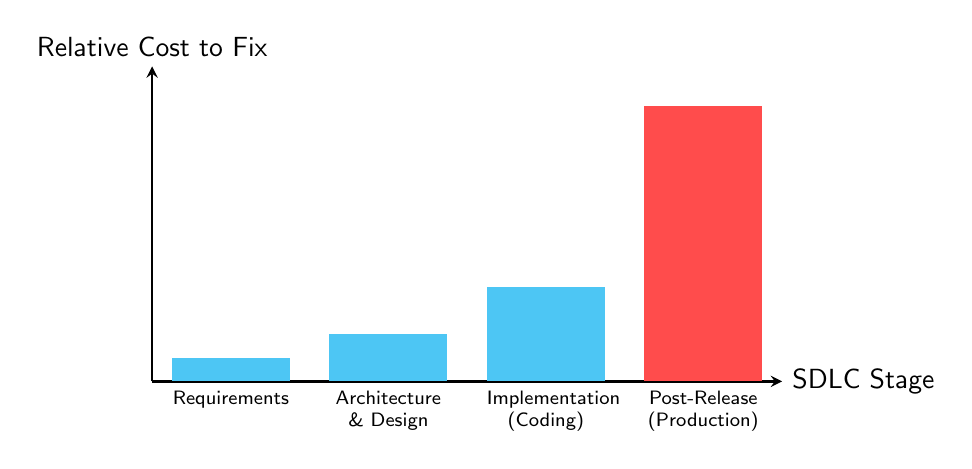
\begin{tikzpicture}[
        bar/.style={rectangle, fill=cyan!70, thick, minimum width=1.5cm, align=center},
        axis/.style={->, >=stealth, thick}
    ]
        % Axes
        \draw[axis] (0,0) -- (8,0) node[right] {SDLC Stage};
        \draw[axis] (0,0) -- (0,4) node[above] {Relative Cost to Fix};
        
        % Bars
        \node[bar, minimum height=0.3cm] at (1, 0.15) {};
        \node[below, font=\scriptsize, text width=1.5cm, align=center] at (1, 0) {Requirements};
        
        \node[bar, minimum height=0.6cm] at (3, 0.3) {};
        \node[below, font=\scriptsize, text width=1.5cm, align=center] at (3, 0) {Architecture\\\& Design};
        
        \node[bar, minimum height=1.2cm] at (5, 0.6) {};
        \node[below, font=\scriptsize, text width=1.5cm, align=center] at (5, 0) {Implementation\\(Coding)};
        
        \node[bar, minimum height=3.5cm, fill=red!70] at (7, 1.75) {};
        \node[below, font=\scriptsize, text width=1.5cm, align=center] at (7, 0) {Post-Release\\(Production)};
    \end{tikzpicture}
\end{frame}

%------------------------------------------------------------
\section{Testing Levels}
%------------------------------------------------------------

\begin{frame}
    \frametitle{Testing Levels (The V-Model)}
    Testing is not a single phase; it occurs at multiple levels, mapping directly to how the software was designed.
    
    \begin{enumerate}
        \item \textbf{Unit Testing:} Tests individual components or functions in isolation. Usually written by the developers themselves.
        \item \textbf{Integration Testing:} Tests how different modules or services work when combined (e.g., Does the Python backend correctly parse JSON from the Robot API?).
        \item \textbf{System Testing:} Evaluates the complete, fully integrated software product to ensure it meets technical specifications.
        \item \textbf{Acceptance Testing:} Conducted by the end-users or clients to verify that the system satisfies the business requirements (Does it actually solve the problem?).
    \end{enumerate}
\end{frame}

\begin{frame}[fragile]
    \frametitle{Zooming in: Unit Testing}
    Unit tests check the smallest testable parts of an application. They should be fast, isolated, and deterministic.
    
    \vspace{0.2cm}
    \textbf{Example (Python using \texttt{pytest}):}
    \begin{minted}[bgcolor=lightgray, fontsize=\scriptsize]{python}
# core_logic.py
def is_valid_coordinate(x, y):
    if x < 0 or y < 0:
        return False
    return True

# test_core_logic.py
def test_is_valid_coordinate():
    # Arrange & Act
    valid = is_valid_coordinate(5, 10)
    invalid = is_valid_coordinate(-1, 5)
    
    # Assert
    assert valid == True
    assert invalid == False
    \end{minted}
    \vspace{0.2cm}
    \footnotesize \textit{If another developer later breaks the \texttt{is\_valid\_coordinate} logic, this test will immediately fail, preventing a bug from reaching production.}
\end{frame}

%------------------------------------------------------------
\section{Testing Types}
%------------------------------------------------------------

\begin{frame}
    \frametitle{Testing Types: Functional vs. Non-Functional}
    We divide testing into \textit{what} the system does versus \textit{how well} it does it.
    
    \begin{block}{Functional Testing}
        Validates the software against functional requirements. 
        \begin{itemize}
            \item \textbf{Examples:} Can the user log in? Does the "Emergency Stop" button halt the robot? Does the database save the audit log?
        \item \textbf{Smoke Testing:} A subset of functional tests to check if the crucial functions work before doing a deeper test pass.
        \end{itemize}
    \end{block}
    
    \begin{block}{Non-Functional Testing}
        Evaluates the operational aspects of the system.
        \begin{itemize}
            \item \textbf{Performance Testing:} How does the backend handle 1,000 simultaneous robot status requests?
            \item \textbf{Security Testing:} Can a user bypass the RBAC controls?
            \item \textbf{Usability Testing:} HCI checks (as discussed in Week 6).
        \end{itemize}
    \end{block}
\end{frame}

\begin{frame}
    \frametitle{Regression Testing}
    \textbf{Definition:} Re-running functional and non-functional tests to ensure that previously developed and tested software still performs after a change.
    
    \vspace{0.3cm}
    \begin{itemize}
        \item As your codebase grows, adding a new feature often accidentally breaks an old one (a "regression").
        \item Manual regression testing is incredibly tedious and error-prone.
        \item \textbf{Solution:} Automated test suites. Every time you commit code to GitHub, the automated runner executes the entire regression suite in seconds.
    \end{itemize}
\end{frame}

%------------------------------------------------------------
\section{Test Automation \& CI/CD}
%------------------------------------------------------------

\begin{frame}
    \frametitle{The Test Automation Pyramid}
    How should we distribute our automated testing efforts?
    
    \vspace{0.2cm}
    \centering
    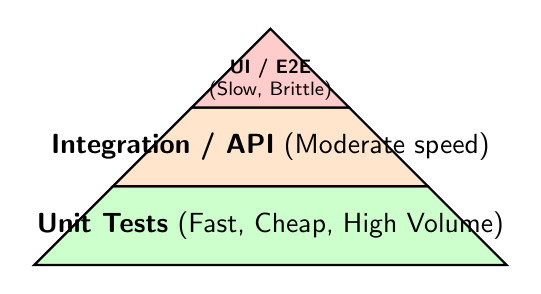
\begin{tikzpicture}
        % Pyramid base (Unit)
        \filldraw[fill=green!20, draw=black, thick] (-3,0) -- (3,0) -- (2,1) -- (-2,1) -- cycle;
        \node at (0,0.5) {\textbf{Unit Tests} (Fast, Cheap, High Volume)};
        
        % Middle tier (Integration)
        \filldraw[fill=orange!20, draw=black, thick] (-2,1) -- (2,1) -- (1,2) -- (-1,2) -- cycle;
        \node at (0,1.5) {\textbf{Integration / API} (Moderate speed)};
        
        % Top tier (UI/E2E)
        \filldraw[fill=red!20, draw=black, thick] (-1,2) -- (1,2) -- (0,3) -- cycle;
        \node[font=\scriptsize, align=center] at (0,2.35) {\textbf{UI / E2E}\\(Slow, Brittle)};
    \end{tikzpicture}
    
    \vspace{0.2cm}
    \begin{itemize}
        \item Write \textbf{lots} of Unit tests (they execute in milliseconds).
        \item Write \textbf{some} Integration tests (they require databases/containers to spin up).
        \item Write \textbf{few} End-to-End UI tests (they require simulating a real browser, which is slow and prone to breaking on minor visual changes).
    \end{itemize}
\end{frame}

\begin{frame}
    \frametitle{Bringing it all together: CI / CD}
    \textbf{Continuous Integration (CI):} The practice of frequently merging code changes into a central repository, where automated builds and tests are run.
    
    \textbf{Continuous Deployment (CD):} Automating the release of validated code to a production environment.
    
    \vspace{0.3cm}
    \textbf{How it works in your project (GitHub Actions):}
    \begin{enumerate}
        \item You push code to GitHub.
        \item GitHub spins up an isolated server.
        \item It builds your \textbf{Docker Containers} (what you learned last week!).
        \item It runs your \textbf{Automated Test Suite} (what you learned today!).
        \item If tests pass, it merges the code. If tests fail, it blocks the merge.
    \end{enumerate}
\end{frame}

%------------------------------------------------------------
\section{Next Steps}
%------------------------------------------------------------

\begin{frame}
    \frametitle{This Week's Lab: Writing Tests \& CI}
    In the workshop, you will implement automated testing for your Assessment 1 Robot Management System.
    
    \begin{itemize}
        \item \textbf{Task 1: Unit Testing:} Write isolated tests for your backend logic (e.g., verifying RBAC permissions or coordinate math).
        \item \textbf{Task 2: API Testing:} Write tests to verify your backend routes return the correct JSON HTTP status codes.
        \item \textbf{Task 3: GitHub Actions CI:} Create a YAML pipeline to automatically run your tests every time you push to your repository.
    \end{itemize}
\end{frame}

\begin{frame}
    \frametitle{Reading \& Resources}
    \begin{itemize}
        \item \textbf{Recommended Reading:} 
        Sommerville, \textit{Software Engineering 9th Edition}, Chapters 8 (Testing) and 25 (Configuration Management).
        \item \textbf{PyTest Documentation:} Excellent starting point if you are writing a Python backend.
        \item \textbf{Jest Documentation:} The industry standard if you are writing a Node.js/JavaScript backend.
        \item \textbf{GitHub Actions Docs:} Review the syntax for creating CI workflows.
    \end{itemize}
\end{frame}

\begin{frame}
    \frametitle{Q \& A}
    \begin{center}
        \Huge Any Questions?\\\vspace{0.5cm} 
        \normalsize fdelduchetto@lincoln.ac.uk
    \end{center}
\end{frame}

\end{document}